\documentclass{beamer}\usepackage[]{graphicx}\usepackage[]{color}
%% maxwidth is the original width if it is less than linewidth
%% otherwise use linewidth (to make sure the graphics do not exceed the margin)
\makeatletter
\def\maxwidth{ %
  \ifdim\Gin@nat@width>\linewidth
    \linewidth
  \else
    \Gin@nat@width
  \fi
}
\makeatother

\definecolor{fgcolor}{rgb}{0.345, 0.345, 0.345}
\newcommand{\hlnum}[1]{\textcolor[rgb]{0.686,0.059,0.569}{#1}}%
\newcommand{\hlstr}[1]{\textcolor[rgb]{0.192,0.494,0.8}{#1}}%
\newcommand{\hlcom}[1]{\textcolor[rgb]{0.678,0.584,0.686}{\textit{#1}}}%
\newcommand{\hlopt}[1]{\textcolor[rgb]{0,0,0}{#1}}%
\newcommand{\hlstd}[1]{\textcolor[rgb]{0.345,0.345,0.345}{#1}}%
\newcommand{\hlkwa}[1]{\textcolor[rgb]{0.161,0.373,0.58}{\textbf{#1}}}%
\newcommand{\hlkwb}[1]{\textcolor[rgb]{0.69,0.353,0.396}{#1}}%
\newcommand{\hlkwc}[1]{\textcolor[rgb]{0.333,0.667,0.333}{#1}}%
\newcommand{\hlkwd}[1]{\textcolor[rgb]{0.737,0.353,0.396}{\textbf{#1}}}%
\let\hlipl\hlkwb

\usepackage{framed}
\makeatletter
\newenvironment{kframe}{%
 \def\at@end@of@kframe{}%
 \ifinner\ifhmode%
  \def\at@end@of@kframe{\end{minipage}}%
  \begin{minipage}{\columnwidth}%
 \fi\fi%
 \def\FrameCommand##1{\hskip\@totalleftmargin \hskip-\fboxsep
 \colorbox{shadecolor}{##1}\hskip-\fboxsep
     % There is no \\@totalrightmargin, so:
     \hskip-\linewidth \hskip-\@totalleftmargin \hskip\columnwidth}%
 \MakeFramed {\advance\hsize-\width
   \@totalleftmargin\z@ \linewidth\hsize
   \@setminipage}}%
 {\par\unskip\endMakeFramed%
 \at@end@of@kframe}
\makeatother

\definecolor{shadecolor}{rgb}{.97, .97, .97}
\definecolor{messagecolor}{rgb}{0, 0, 0}
\definecolor{warningcolor}{rgb}{1, 0, 1}
\definecolor{errorcolor}{rgb}{1, 0, 0}
\newenvironment{knitrout}{}{} % an empty environment to be redefined in TeX

\usepackage{alltt}
\usepackage{standalone}
\standalonetrue
\ifstandalone
  \usepackage{../haziq_beamer}
  \addbibresource{../bib/phd-presentation-3.bib}
\fi





\IfFileExists{upquote.sty}{\usepackage{upquote}}{}
\begin{document}

\ifstandalone
  \section{Examples}
\fi

\subsection*{Fisher's Iris data set}

\begin{frame}[fragile]{Fisher's Iris data set}
\begin{knitrout}\small
\definecolor{shadecolor}{rgb}{0.969, 0.969, 0.969}\color{fgcolor}

{\centering 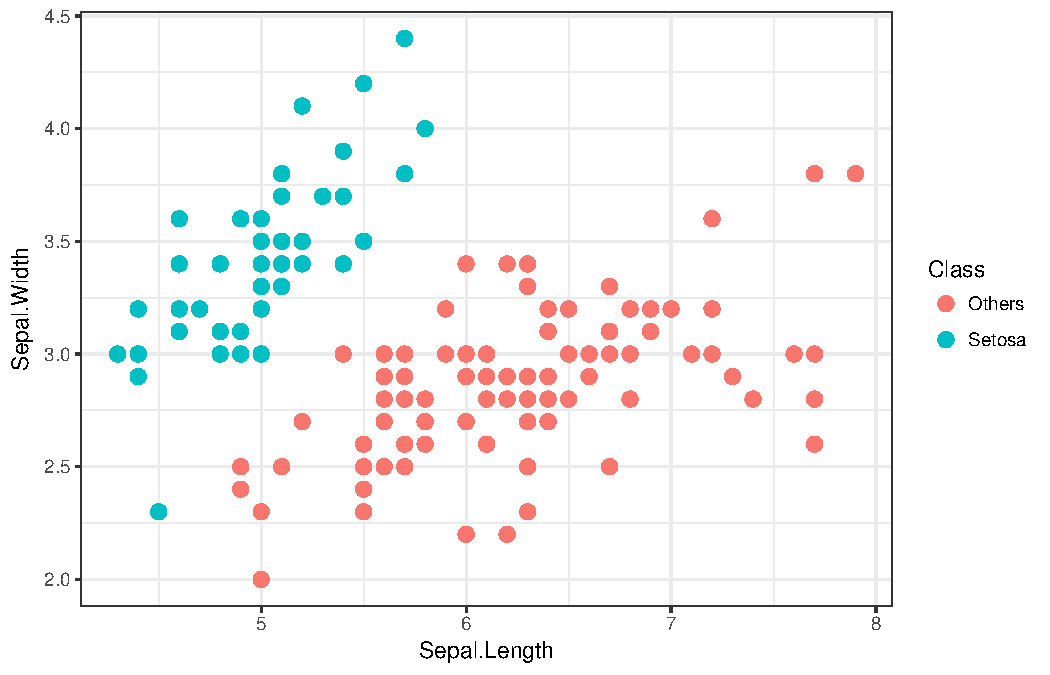
\includegraphics[width=\maxwidth]{figure/data_iris-1} 

}



\end{knitrout}
\end{frame}


\begin{frame}[fragile]{Fisher's Iris data set - Model fitting}
\blfootnote{\fullcite{Jamil2017iprobit}}
\vspace{-13pt}
\begin{itemize}
\item Varitional inference for I-prior probit models implemented in \proglang{R} package \pkg{iprobit} (still lots of work to do!).
\end{itemize}
\begin{knitrout}\small
\definecolor{shadecolor}{rgb}{0.969, 0.969, 0.969}\color{fgcolor}\begin{kframe}
\begin{alltt}
\hlstd{R> }\hlkwd{system.time}\hlstd{(}
\hlstd{+ }  \hlstd{(mod} \hlkwb{<-} \hlkwd{iprobit}\hlstd{(y, X))}
\hlstd{+ }\hlstd{)}
\end{alltt}
\end{kframe}
\end{knitrout}
\vspace{-25pt}
\begin{knitrout}\small
\definecolor{shadecolor}{rgb}{0.969, 0.969, 0.969}\color{fgcolor}\begin{kframe}
\begin{alltt}
\vspace{0.8em}
\end{alltt}
\end{kframe}
\end{knitrout}
\vspace{-25pt}
\begin{knitrout}\small
\definecolor{shadecolor}{rgb}{0.969, 0.969, 0.969}\color{fgcolor}\begin{kframe}
\begin{verbatim}
## 
## |=================================                     |  61%
##  Converged after 6141 iterations.
##  Training error rate: 0 %
##     user  system elapsed
##   67.857   6.396  74.277
\end{verbatim}
\end{kframe}
\end{knitrout}

\end{frame}

\begin{frame}[fragile]{Fisher's Iris data set - Model summary}
\begin{knitrout}\small
\definecolor{shadecolor}{rgb}{0.969, 0.969, 0.969}\color{fgcolor}\begin{kframe}
\begin{alltt}
\hlstd{R> }\hlkwd{summary}\hlstd{(mod)}
\end{alltt}
\begin{verbatim}
## 
## Call:
## iprobit(y = y, X, maxit = 10000)
## 
## RKHS used: Canonical 
## 
##           Mean   S.D.    2.5%   97.5%
## alpha  -4.1730 0.0816 -4.3330 -4.0129
## lambda  1.2896 0.0142  1.2618  1.3175
## 
## Converged to within 1e-05 tolerance. No. of iterations: 6141
## Model classification error rate (%): 0
## Variational lower bound: -12.93486
\end{verbatim}
\end{kframe}
\end{knitrout}
\end{frame}

\begin{frame}[fragile]{Fisher's Iris data set - Lower bound}
\vspace{-7pt}
\begin{knitrout}\small
\definecolor{shadecolor}{rgb}{0.969, 0.969, 0.969}\color{fgcolor}\begin{kframe}
\begin{alltt}
\hlstd{R> }\hlkwd{iplot_lb}\hlstd{(mod,} \hlkwc{niter.plot} \hlstd{=} \hlnum{10}\hlstd{)}
\end{alltt}
\end{kframe}
\end{knitrout}
\begin{knitrout}\small
\definecolor{shadecolor}{rgb}{0.969, 0.969, 0.969}\color{fgcolor}

{\centering 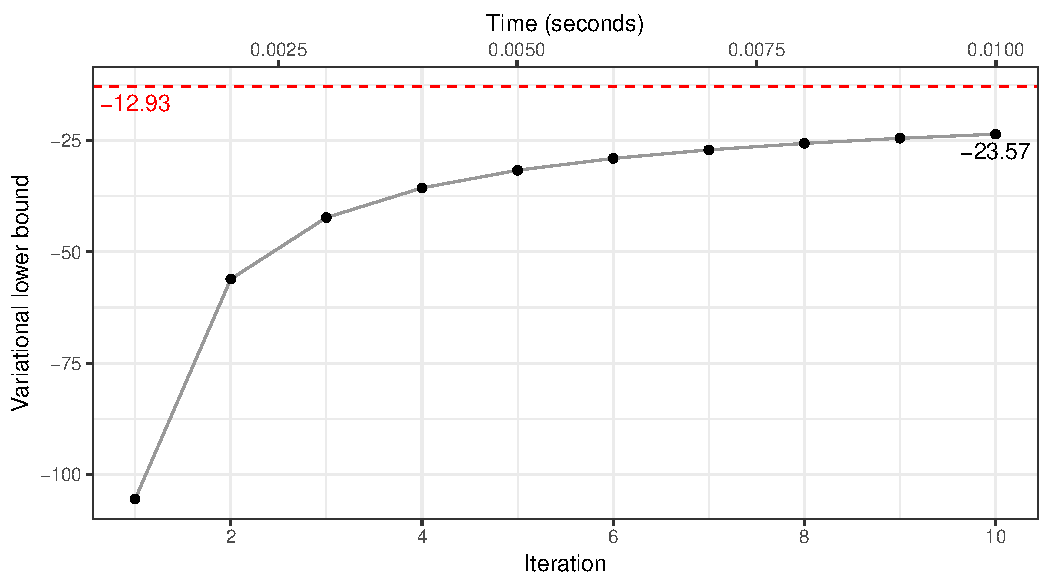
\includegraphics[width=\maxwidth]{figure/iris-lb-1} 

}



\end{knitrout}
\end{frame}

\begin{frame}[fragile]{Fisher's Iris data set - Decision boundary}
\vspace{-5pt}
\begin{knitrout}\small
\definecolor{shadecolor}{rgb}{0.969, 0.969, 0.969}\color{fgcolor}\begin{kframe}
\begin{alltt}
\hlstd{R> }\hlkwd{iplot_decbound}\hlstd{(mod)}
\end{alltt}
\end{kframe}

{\centering 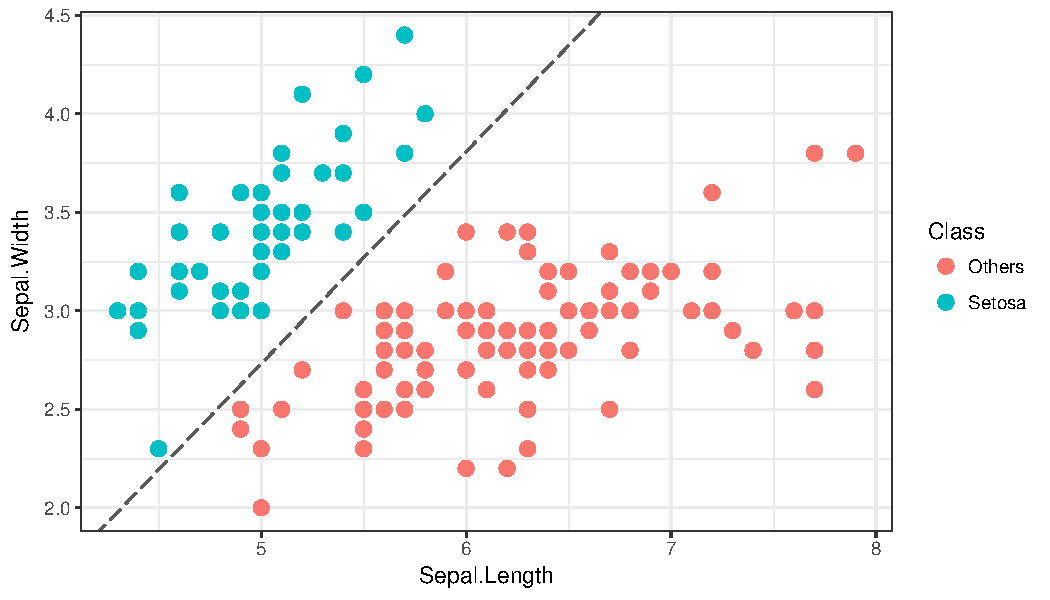
\includegraphics[width=\maxwidth]{figure/iris-decbound-1} 

}



\end{knitrout}
\end{frame}

\subsection*{Cardiac arrhythmia data set}

\begin{frame}[fragile]{Cardiac arrhythmia data set}
\blfootnote{\fullcite{ArrhythmiaData}}
\vspace{-20pt}
\begin{itemize}
% \item Original data set contains 16 classes of arrhythmia .
\item Detect the presence of cardiac arrhythmia based on various ECG data and other attributes such as age and weight ($n = 451, p = 194$).
\end{itemize}

\begin{knitrout}\small
\definecolor{shadecolor}{rgb}{0.969, 0.969, 0.969}\color{fgcolor}

{\centering 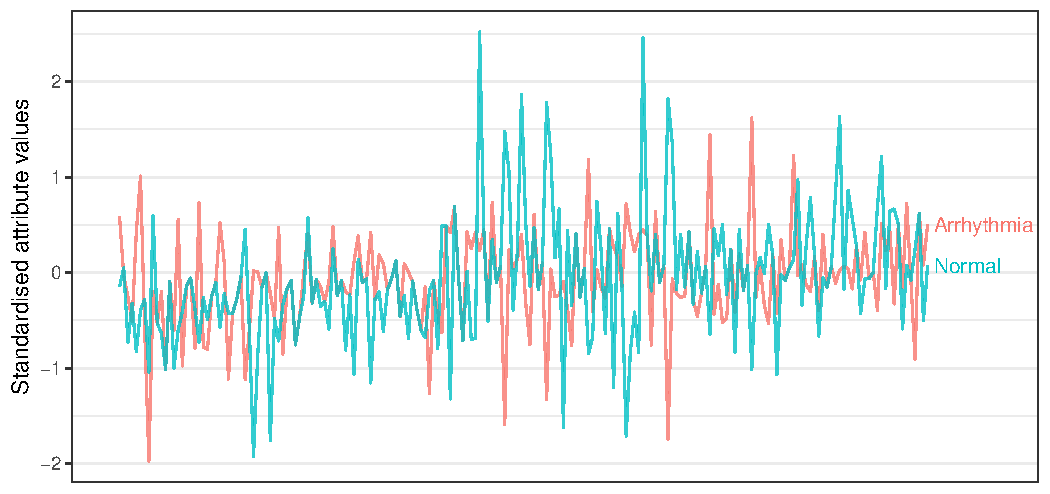
\includegraphics[width=\maxwidth]{figure/plot_cardiac-1} 

}



\end{knitrout}
\end{frame}


\begin{frame}[fragile]{Cardiac arrhythmia data set - Model fit}
\blfootnote{\fullcite{Cannings2017}}
\vspace{-20pt}
\begin{itemize}
  \item Fit an I-prior probit model using Canonical and FBM kernels. The full data set takes about 35 seconds.
\end{itemize}
\vspace{-5pt}
\begin{knitrout}\small
\definecolor{shadecolor}{rgb}{0.969, 0.969, 0.969}\color{fgcolor}\begin{kframe}
\begin{alltt}
\hlstd{R> }\hlstd{mod} \hlkwb{<-} \hlkwd{iprior}\hlstd{(y, X,} \hlkwc{kernel} \hlstd{=} \hlstr{"FBM"}\hlstd{)}
\end{alltt}
\end{kframe}
\end{knitrout}
\vspace{-10pt}
\begin{itemize}
  \item Compare against popular classifiers: 1) $k$-nearest neighbours; 2) support vector machine; 3) Gaussian process classification; 4) random forests; 5) nearest shrunken centroids \parencite{tibshirani2003class}; and 6) L-1 penalised logistic regression.
  \vspace{0.5em}
  \item Experiment set-up:
  \begin{itemize}
    \item Form training set by sub-sampling $n_{\text{sub}} \in \{50, 100, 200 \}$ data points.
    \item Use remaining data as test set.
    \item Fit model on training set and obtain test error rates.
    \item Repeat 100 times.
  \end{itemize}
\end{itemize}

\end{frame}


\begin{frame}[fragile]{Cardiac arrhythmia data set - Results}
\begin{knitrout}\small
\definecolor{shadecolor}{rgb}{0.969, 0.969, 0.969}\color{fgcolor}

{\centering 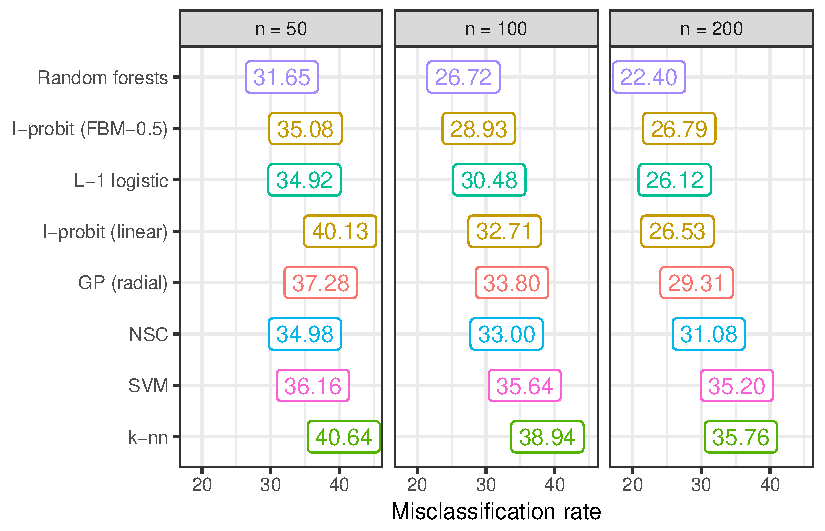
\includegraphics[width=\maxwidth]{figure/cardiac-res-plot-1} 

}



\end{knitrout}
\end{frame}

\subsection*{Meta-analysis of smoking cessation}


\begin{frame}[fragile]{Meta-analysis of smoking cessation}
  \blfootnote{\fullcite[§9.5]{Skrondal2004}}
  \vspace{-30pt}

  \definecolor{col1}{HTML}{F8766D}
  \definecolor{col2}{HTML}{D89000}
  \definecolor{col3}{HTML}{A3A500}
  \definecolor{col4}{HTML}{39B600}
  \definecolor{col5}{HTML}{00BF7D}
  \definecolor{col6}{HTML}{00BFC4}
  \definecolor{col7}{HTML}{00B0F6}
  \definecolor{col8}{HTML}{9590FF}
  \definecolor{col9}{HTML}{E76BF3}
  \definecolor{col10}{HTML}{FF62BC}
  \newcommand{\ebx}{{\color{white} 1\hspace{-20pt}}}
  \begin{center}
  \begin{forest}
  %where n children=0{}{},
  for tree={
    edge path={
      \noexpand\path[\forestoption{edge}]
        (!u.parent anchor) -- +(0,-13pt) -|
        (.child anchor)\forestoption{edge label};
    },
    l sep=5pt, s sep=0pt
  }
  [
    [{\color{col2}\footnotesize Fagerstrom 1982}
      [\ebx] [\ebx] [\ebx] [\ebx] [\ebx] [\ebx]
    ]
    [{\color{col10}\footnotesize Villa 1999}
      [\ebx] [\ebx] [\ebx] [\ebx] [\ebx]
    ]
    [{\color{col7}\footnotesize Nakamura 1990}
      [\ebx] [\ebx] [\ebx]
    ]
    [{\color{col4}\footnotesize Garvey 2000}
      [\ebx] [\ebx] [\ebx] [\ebx]
    ]
    [$\cdots$]
    [{\color{col8}\footnotesize Niaura 1999}
      [\ebx] [\ebx] [\ebx] [\ebx] [\ebx]
    ]
  ]
  \end{forest}
  \end{center}

  \vspace{-25pt}
  \begin{itemize}
    \item Data from 27 separate smoking cessation studies, where participants subjected to nicotine gum treatment or placed in control group.
    \item Some summary statistics:
  \end{itemize}

\begin{center}

\begin{tabular}{l|r|r|r|r|r}
\hline
  & Min. & Avg. & Max. & Prop. quit & Odds quit\\
\hline
Control & 20 & 101 & 617 & 0.207 & 0.261\\
\hline
Treated & 21 & 117 & 600 & 0.320 & 0.470\\
\hline
\end{tabular}


\end{center}

  \vspace{-5pt}
  \begin{itemize}
    \item Raw odds ratio: 1.801.
    \item Random-effects analysis using a multilevel logistic model estimates this  odds ratio as 1.768.
  \end{itemize}
  \vspace{4pt}

\end{frame}


\begin{frame}[fragile]{Meta-analysis of smoking cessation - model}
  \begin{itemize}\setlength\itemsep{0.3em}
    \item Let $i = 1,\dots,n_j$ index the patients in study group $j \in 1,\dots,27$.
    \item Denote $y_{ij}$ as the binary response variable indicating \texttt{Quit} (1) or \texttt{Remain} (0), and $x_{ij}$ as $\text{patient}_{ij}$'s treatment group indicator.
    \item Model binary data using I-probit model
    \begin{align*}
      \Phi^{-1}(p_{ij}) &= f(x_{ij}, j) \\
      &= f_1(x_{ij}) + f_2(j) + f_{12}(x_{ij}, j)
    \end{align*}
    with $f_1, f_2 \in$ Pearson RKHS, and $f_{12} \in$ ANOVA RKHS.
  \end{itemize}

\newcolumntype{R}[1]{>{\raggedleft\let\newline\\\arraybackslash\hspace{0pt}}m{#1}}
\begin{center}

\begin{tabular}{l|l|r|r|R{2.2cm}}
\hline
  & Model & Lower bound & Brier score & No. of RKHS\newline param.\\
\hline
1 & $f_1$ & -3210.79 & 0.0311 & 1\\
\hline
2 & $f_1 + f_2$ & -3097.24 & 0.0294 & 2\\
\hline
3 & $f_1 + f_2 + f_{12}$ & -3091.21 & 0.0294 & 2\\
\hline
\end{tabular}


\end{center}

\end{frame}

\begin{frame}[fragile]{Meta-analysis of smoking cessation - results}
\vspace{-3pt}
\begin{knitrout}\small
\definecolor{shadecolor}{rgb}{0.969, 0.969, 0.969}\color{fgcolor}

{\centering 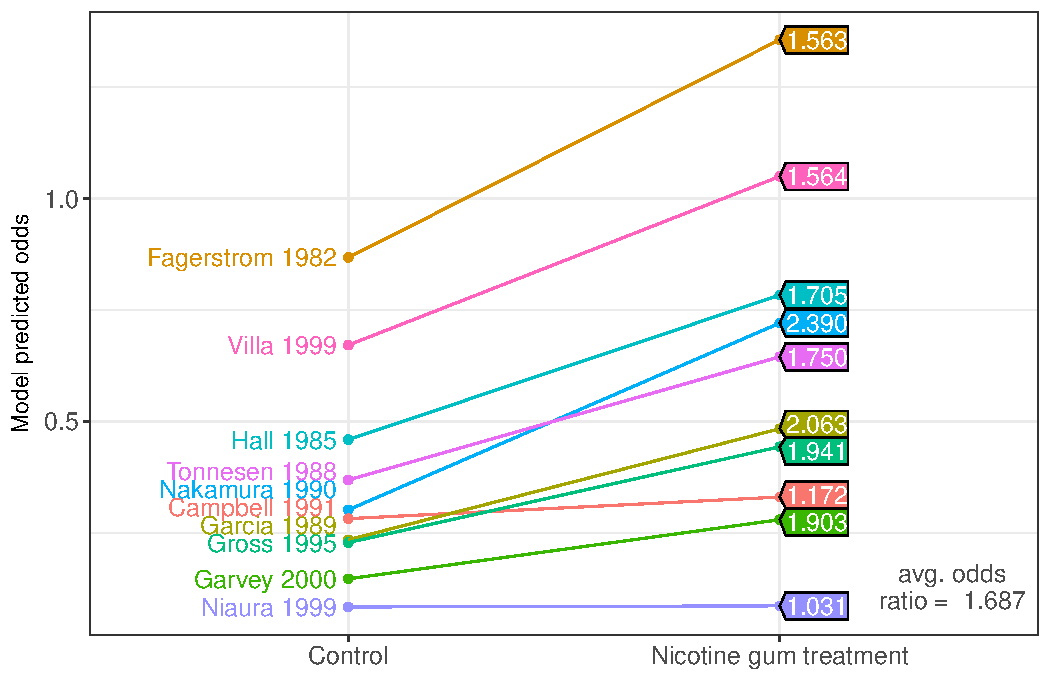
\includegraphics[width=\maxwidth]{figure/plot_smoke-1} 

}



\end{knitrout}
\end{frame}

\end{document}


